\documentclass[10pt,journal,compsoc]{IEEEtran}
%
%
%
\ifCLASSOPTIONcompsoc
  %
  %
  \usepackage[nocompress]{cite}
\else
  %
  \usepackage{cite}
\fi
%
%
\hyphenation{op-tical net-works semi-conduc-tor}
\usepackage{graphicx}
\usepackage{amsmath}
\usepackage{amssymb, url}
\urlstyle{sf}
%
\usepackage{bm}
\usepackage[usenames]{color}
\usepackage{icomma}
%
\usepackage[ruled,lined]{algorithm2e}
\usepackage[svgnames,table]{xcolor}
\usepackage{makecell}
\usepackage{booktabs}
\usepackage{multirow}
\usepackage[bf,font=footnotesize]{caption}
\usepackage{array}
\usepackage{wrapfig}

\newcommand{\etal}{\emph{et al.}}
\newcommand{\eg}{\emph{e.g.}}
\newcommand{\etc}{\emph{etc.}}
\newcommand{\ie}{\emph{i.e.}}
\newcommand{\cf}{\emph{c.f.}}
\newcommand{\itm}{a}
\renewcommand{\i}{{\itm}}
\newcommand{\vs}{\emph{vs.}}
%
%
\def\Att{{V_{att}}}
\def\Cap{{V_{cap}}}
\def\Know{{V_{know}}}
\def\V2L{\textit{V2L}}
\def\CNN{\mbox{CNN}}
\def\ModParms{{\boldsymbol \theta}}



\begin{document}
%
\title{Image Captioning and Visual Question Answering Based on Attributes
%
\\and External Knowledge}
%
%
%
\author{Qi Wu, Chunhua Shen,  Peng Wang, Anthony Dick, Anton van den Hengel
\IEEEcompsocitemizethanks{\IEEEcompsocthanksitem
  The authors are with the Australian Centre for Visual Technologies, and  School of Computer Science,
  at The University of Adelaide, Australia.
 %
 %
 %
 %
  E-mail: (\{qi.wu01, chunhua.shen, p.wang, anthony.dick, anton.vandenhengel\}@\-adelaide.\-edu.\-au).
}
}





\markboth{Manuscript, 2016}%
{}

\IEEEtitleabstractindextext{%

\begin{abstract}
Much of the recent progress in Vision-to-Language problems has been achieved through a combination of Convolutional Neural Networks (CNNs)
and Recurrent Neural Networks (RNNs). This approach does not explicitly represent high-level semantic concepts, but rather seeks to progress directly from image features to text. In this paper we first propose a method of incorporating high-level concepts into the successful CNN-RNN approach, and show that it achieves a significant improvement on the state-of-the-art in both image captioning and visual question answering.
We further show that the same mechanism can be used to incorporate external knowledge,
which is critically important for answering high level visual questions.
Specifically, we design a visual question answering model that combines an internal representation of the content of an
image with information extracted from a general knowledge base to answer a broad range of image-based questions.
It particularly allows questions to be asked 
%
where the image alone does not contain the the information required to select the appropriate answer.
%
Our final model achieves the best reported results for both image captioning and visual question answering on several of the major benchmark datasets.
\end{abstract}


%
\begin{IEEEkeywords}
  Image Captioning, Visual Question Answering, Concepts Learning, Recurrent Neural Networks, LSTM.
\end{IEEEkeywords}}
%
\maketitle

\IEEEdisplaynontitleabstractindextext
\IEEEpeerreviewmaketitle



%
\section{Introduction}
\label{sec:introduction}
\section{Introduction}
\label{sec:intro}

Language modeling is among the important problems that require modeling long-term dependency, with successful applications such as unsupervised pretraining~\citep{dai2015semi,peters2018deep,radford2018improving,devlin2018bert}.
However, it has been a challenge to equip neural networks with the capability to model long-term dependency in sequential data.
Recurrent neural networks (RNNs), in particular Long Short-Term Memory (LSTM) networks~\citep{hochreiter1997long}, have been a standard solution to language modeling and obtained strong results on multiple benchmarks.
Despite the wide adaption, RNNs are difficult to optimize due to gradient vanishing and explosion~\citep{hochreiter2001gradient}, and the introduction of gating in LSTMs and the gradient clipping technique~\citep{graves2013generating} might not be sufficient to fully address this issue.
% ,pascanu2012understanding
Empirically, previous work has found that LSTM language models use 200 context words on average~\citep{khandelwal2018sharp}, indicating room for further improvement.

On the other hand, the direct connections between long-distance word pairs baked in attention mechanisms might ease optimization and enable the learning of long-term dependency~\citep{bahdanau2014neural,vaswani2017attention}.
Recently, \citet{al2018character} designed a set of auxiliary losses to train deep Transformer networks for character-level language modeling, which outperform LSTMs by a large margin.
Despite the success, the LM training in~\citet{al2018character} is performed on separated fixed-length segments of a few hundred characters, without any information flow across segments.
As a consequence of the fixed context length, the model cannot capture any longer-term dependency beyond the predefined context length.
In addition, the fixed-length segments are created by selecting a consecutive chunk of symbols without respecting the sentence or any other semantic boundary.
Hence, the model lacks necessary contextual information needed to well predict the first few symbols, leading to inefficient optimization and inferior performance.
We refer to this problem as \textit{context fragmentation}.

%However, the context length is fixed to hundreds of characters and thus it is not possible to model longer-term dependency. Moreover, it is not clear how the model performs on word-level language modeling data, as the granularity changes.

% Moreover, using auxiliary losses brings additional challenges such as properly tuning the mixture weights and the loss decay schedule.

To address the aforementioned limitations of fixed-length contexts, we propose a new architecture called Transformer-XL (meaning extra long).
We introduce the notion of recurrence into our deep self-attention network. In particular, instead of computing the hidden states from scratch for each new segment, we reuse the hidden states obtained in previous segments.
The reused hidden states serve as memory for the current segment, which builds up a recurrent connection between the segments.
As a result, modeling very long-term dependency becomes possible because information can be propagated through the recurrent connections.
Meanwhile, passing information from the previous segment can also resolve the problem of context fragmentation.
More importantly, we show the necessity of using relative positional encodings rather than absolute ones, in order to enable state reuse without causing temporal confusion.
Hence, as an additional technical contribution, we introduce a simple but more effective relative positional encoding formulation that generalizes to attention lengths longer than the one observed during training.

Transformer-XL obtained strong results on five datasets, varying from word-level to character-level language modeling.
Transformer-XL is also able to generate relatively coherent long text articles with \textit{thousands of} tokens (see Appendix \ref{sec:gen}), trained on only 100M tokens.
% Transformer-XL improves the previous state-of-the-art (SoTA) results from 1.06 to 0.99 in bpc on enwiki8, from 1.13 to 1.08 in bpc on text8, from 20.5 to 18.3 in perplexity on WikiText-103, and from 23.7 to 21.8 in perplexity on One Billion Word.
% Transformer-XL improves the previous state-of-the-art (SoTA) results to 0.99 in bpc on enwiki8, 1.08 in bpc on text8, 18.3 in perplexity on WikiText-103, and 21.8 in perplexity on One Billion Word.
% On small data, Transformer-XL also achieves a perplexity of 54.5 on Penn Treebank without finetuning, which is SoTA when comparable settings are considered.

Our main technical contributions include introducing the notion of recurrence in a purely self-attentive model and deriving a novel positional encoding scheme. These two techniques form a complete set of solutions, as any one of them alone does not address the issue of fixed-length contexts. Transformer-XL is the first self-attention model that achieves substantially better results than RNNs on both character-level and word-level language modeling.

% On WikiText-103, Transformer-XL improves the previous state-of-the-art (SoTA) results from 33 perplexity to 24, with a relative reduction of 27\%. On enwiki8 character-level language modeling, Transformer-XL achieves a SoTA bpc of 1.03, which outperforms \cite{al2018character} by 0.03 with 60+\% fewer parameters. Given a more common model size with 40+M parameters, Transformer-XL achieves a bpc of 1.06, compared to 1.11 by \cite{al2018character}. Transformer-XL also achieves perplexities of 54.5 on Penn Treebank and 29.4 on One Billion Word, which are SoTA when comparable settings are considered.

% Due to the ability of modeling long-range context, our best model uses attention lengths of 1,600 and 3,800 on WikiText-103 and enwiki8 respectively. We also devise a metric called \textit{Relative Effective Context Length} (RECL) that aims to fairly compare the ability of long-range dependency modeling.
% % perform a fair comparison of the gains brought by increasing the context lengths for different models.
% In this setting, Transformer-XL learns a RECL of 900 words on WikiText-103, while the numbers for recurrent networks and Transformer are only 500 and 128.

% We use two methods to quantitatively study the effective lengths of Transformer-XL and the baselines. Similar to \cite{khandelwal2018sharp}, we gradually increase the attention length at test time until no further noticeable improvement ($\sim$0.1\% relative gains) can be observed. Our best model in this settings use attention lengths of 1,600 and 3,800 on WikiText-103 and enwiki8 respectively.
% %In addition, since the effective context length of Transformer-XL can be longer than the attention length due to our recurrent formulation, we devise a metric called \textit{Relative Effective Context Length} (RECL) that aims to perform a fair comparison of the gains brought by increasing the context lengths for different models.
% In addition, we devise a metric called \textit{Relative Effective Context Length} (RECL) that aims to perform a fair comparison of the gains brought by increasing the context lengths for different models.
% In this setting, Transformer-XL learns a RECL of 900 words on WikiText-103, while the numbers for recurrent networks and Transformer are only 500 and 128.


\section{Related work}
\label{sec:related_work}
\subsection{Attribute-based Representation} Using attribute-based models as a high-level representation has shown potential in many computer vision tasks such as object recognition, image annotation and image retrieval. Farhadi \etal \cite{farhadi2009describing} were
among the first to propose to use a set of visual semantic attributes to identify familiar objects, and to describe unfamiliar objects. %
Vogel and Schiele \cite{vogel2007semantic} used visual attributes describing scenes to characterize image regions and combined these local semantics into a global image description. Su \etal \cite{su2012improving} defined six groups of attributes to build intermediate-level features for image classification. Li \etal \cite{li2010object,li2012objects} introduced the concept of an `object bank' which enables objects to be used as attributes for scene representation.

\subsection{Image Captioning} The problem of annotating images with natural language at the scene level has long been studied in both computer vision and natural language processing. Hodosh \etal~\cite{hodosh2013framing} proposed to frame sentence-based image annotation as the task of ranking a given pool of captions. Similarly,~\cite{gong2014improving,jia2011learning,ordonez2011im2text} posed the task as a retrieval problem, but based on co-embedding of images and text in the same space. Recently, Socher \etal \cite{socher2014grounded} used neural networks to co-embed image and sentences together and Karpathy \etal~\cite{karpathy2014deep} co-embedded image crops and sub-sentences. %

Attributes have been used in many image captioning methods to fill the gaps in predetermined caption templates. Farhadi \etal~\cite{farhadi2010every}, for instance, used detections to infer a triplet of scene elements which is converted to text using a template. Li \etal \cite{li2011composing} composed image descriptions given computer vision based inputs such as detected objects, modifiers and locations using web-scale $n$-grams. Zhu \etal \cite{yao2010i2t} converted image parsing results into a semantic representation in the form of Web Ontology Language, which is converted to human readable text. A more sophisticated CRF-based method use of attribute detections beyond triplets was proposed by Kulkarni \textit{et al} \cite{kulkarni2013babytalk}. The advantage of template-based methods is that the resulting captions are more likely to be grammatically correct. The drawback is that they still rely on hard-coded visual concepts and suffer the implied limits on the variety of the output. %
Fang \etal \cite{fang2014captions} won the 2015 COCO Captioning Challenge with an approach that is similar to ours in as much as it applies a visual concept (i.e., attribute) detection process before generating sentences. They first learned $1000$ independent detectors for visual words based on a multi-instance learning framework and then used a maximum entropy language model conditioned on the set of visually detected words directly to generate captions. 
%
%
%

In contrast to the aforementioned two-stage methods, the recent dominant trend in \V2L is to use an architecture which connects a CNN to an RNN to learn the mapping from images to sentences directly. Mao \etal \cite{mao2014deep}, for instance, proposed a multimodal RNN (m-RNN) to estimate the probability distribution of the next word given previous words and the deep CNN feature of an image at each time step. Similarly, Kiros \etal \cite{kiros2014unifying} constructed a joint multimodal embedding space using a powerful deep CNN model and an LSTM that encodes text. Karpathy and Li \cite{Karpathy2014deepvs} also proposed a multimodal RNN generative model, but in contrast to \cite{mao2014deep}, their RNN is conditioned on the image information only at the first time step. Vinyals \etal \cite{vinyals2014show} combined deep CNNs for image classification with an LSTM for sequence modeling, to create a single network that generates descriptions of images. Chen \etal \cite{Chen2015CVPRMind} learn a bi-directional mapping between images and their sentence-based descriptions, which allows to reconstruct visual features given an image description. Xu \etal \cite{xu2015show} proposed a model based on visual attention. Jia \etal \cite{jia2015guilding} applied additional retrieved sentences to guide the LSTM in generating captions.

Interestingly, this end-to-end CNN-RNN approach ignores the image-to-word mapping which was an essential step in many of the previous image captioning systems detailed above~\cite{farhadi2010every,kulkarni2013babytalk,li2011composing,yang2011corpus}. The CNN-RNN approach has the advantage that it is able to generate a wider variety of captions, can be trained end-to-end, and outperforms the previous approach on the benchmarks. It is not clear, however, what the impact of bypassing the intermediate high-level representation is, and particularly to what extent the RNN language model might be compensating. Donahue \etal \cite{donahue2014long} described an experiment, for example, using tags and CRF models as a mid-layer representation for video to generate descriptions, but it was designed to prove that LSTM outperforms an SMT-based approach \cite{rohrbach2013translating}. It remains unclear whether the mid-layer representation or the LSTM leads to the success. Our paper provides several well-designed experiments to answer this question.

We thus here show not only a method for introducing a high-level representation into the CNN-RNN framework, and that doing so improves performance, but we also investigate the value of high-level information more broadly in \V2L tasks.  This is of critical importance at this time because \V2L has a long way to go, particularly in the generality of the images and text it is applicable to.

\begin{figure*}[t!]
  \centering
  \includegraphics[width=0.85\textwidth]{./img/captioning_frame.pdf}\\
  \vspace{-5pt}
  \caption{Our attribute-based image captioning framework. The image analysis module learns a mapping between an image and the semantic attributes through a CNN. The language module learns a mapping from the attributes vector to a sequence of words using an LSTM. }
  \label{img:cap_frame}
  \vspace{-5pt}
\end{figure*}

\subsection{Visual Question Answering} Malinowski \etal \cite{malinowski2014multi}
may be the first to study the VQA problem. They proposed a method that combines semantic parsing and image segmentation with a Bayesian approach to sampling from nearest neighbors in the training set. %
Tu \etal~\cite{tu2014joint} built a query answering system based on a joint parse graph from text and videos. Geman \etal~\cite{geman2015visual} proposed an automatic `query generator' that is trained on annotated images and produces a sequence of binary questions from any given test image. Each of these approaches places significant limitations on the form of question that can be answered.

Most recently, inspired by the significant progress achieved using deep neural network models in both computer vision and natural language processing, an architecture which combines a CNN and RNN to learn the mapping from images to sentences has become the dominant trend. Both Gao \etal~\cite{gao2015you} and Malinowski \etal \cite{malinowski2015ask} used RNNs to encode the question and output the answer.  Whereas Gao \etal~\cite{gao2015you} used two networks, a separate encoder and decoder, Malinowski \etal \cite{malinowski2015ask} used a single network for both encoding and decoding. Ren \etal \cite{ren2015image} focused on questions with a single-word answer and formulated the task as a classification problem using an LSTM. %
Antol \etal \cite{antol2015vqa} proposed a large-scale open-ended VQA dataset based on COCO, which is called VQA. %
Inspired by Xu \etal \cite{xu2015show} who encode visual attention in the Image Captioning, \cite{zhu2015visual7w,xu2015ask,Chen2015ABC,Jiang2015compositional,andreas2015deep,yang2015stacked} propose to use the spatial attention to help answering visual questions. \cite{xu2015ask, yang2015stacked, Noh2015image}
formulate the VQA as a classification problem and restrict the answer only can be drawn from a fixed answer space. %

Our framework also exploits both CNN and RNNs, but in contrast to preceding approaches which use only image features extracted from a CNN in answering a question, we employ multiple sources, including image content, generated image captions and mined external knowledge, to feed to an RNN to answer questions. Large-scale Knowledge Bases (KBs), such as Freebase~\cite{bollacker2008freebase} and DBpedia~\cite{auer2007dbpedia}, have been used successfully in several natural language Question Answering (QA) systems~\cite{berant2013semantic,ferrucci2010building}. However, VQA systems exploiting KBs are still relatively rare.

%
Zhu \etal \cite{zhu2015building} used a hand-crafted KB primarily containing image-related information such as category labels, attribute labels and affordance labels, but also some quantities relating to their specific question format such as GPS coordinates and similar. %
Instead of building a problem-specific KB, we use a pre-built large-scale KB (DBpedia \cite{auer2007dbpedia}) from which we extract information using a standard RDF query language. DBpedia has been created by extracting structured information from Wikipedia, and is thus significantly larger and more general than a hand-crafted KB. Rather than having a user pose their question in a formal query language, our VQA system is able to encode questions written in natural language automatically.  This is achieved without manually specified formalization, but rather depends on processing a suitable training set. The result is a model which is very general in the forms of question that it will accept.
The quality of the information in the KB is one of the primary issues in this approach to VQA. The problem is that KBs constructed by analysing Wikipedia and similar are patchy and inconsistent at best, and hand-curated KBs are inevitably very topic specific. Using visually-sourced information is a promising approach to solve this problem~\cite{Lin_2015_CVPR, Sadeghi_2015_CVPR}, but has a way to go before it might be usefully applied within our approach. After inspecting the database shows that the ‘comment’ field is the most generally informative about an attribute, as it contains a general text description of it. We therefore find this is still a feasible solution. 


\section{Image Captioning using Attributes}
\label{sec:image_captioning}
Our image captioning model is summarized in Figure \ref{img:cap_frame}. The model includes an image analysis part and a caption generation part. In the image analysis part, we first use supervised learning to predict a set of attributes, based on words commonly found in image captions %
We solve this as a \textit{multi-label classification problem} and train a corresponding deep CNN by minimizing an element-wise logistic loss function. Secondly, a fixed length vector $\Att(I)$ is created for each image $I$, whose length is the size of the attribute set. Each dimension of the vector contains the prediction probability for a particular attribute. In the captioning generation part, we apply an LSTM-based sentence generator. In the baseline model, as in~\cite{gao2015you,ren2015image,vinyals2014show} we use a pre-trained CNN to extract image features $\CNN(I)$ which are fed into the LSTM directly. For the sake of completeness a fine-tuned version of this approach is also implemented.

\subsection{Attribute-based Image Representation}
\label{subsec:Attributes_Predictor}
Our first task is to describe the image content in terms of a set of attributes. An attribute vocabulary is first constructed. Unlike~\cite{kulkarni2013babytalk,yang2011corpus}, that use a vocabulary from separate hand-labeled training data, our semantic attributes are extracted from training captions and can be any part of speech, including object names (nouns), motions (verbs) or properties (adjectives). The direct use of captions guarantees that the most salient attributes for an image set are extracted. We use the $c$ ($c=256$) most common words in the training captions to determine the attribute vocabulary $\mathcal{V}_{att}$. Similar to \cite{fang2014captions}, the top $15$ most frequent closed-class words such as \texttt{`a',`on',`of'}  are removed since they are in nearly every caption. In contrast to~\cite{fang2014captions}, our vocabulary is not tense or plurality sensitive, for instance, \texttt{`ride'} and \texttt{`riding'} are classified as the same semantic attribute, similarly \texttt{`bag'} and \texttt{`bags'}. This significantly decreases the size of our attribute vocabulary. The full list of attributes can be found in the supplementary material. Our attributes represent a set of high-level semantic constructs, the totality of which the LSTM then attempts to represent in sentence form. Generating a sentence from a vector of attribute likelihoods exploits a much larger set of candidate words which are learned separately, allowing for greater flexibility in the generated text.

Given this attribute vocabulary, we can associate each image with a set of attributes according to its captions. We then wish to predict the attributes given a test image. Because we do not have ground truth bounding boxes for attributes, we cannot train a detector for each using the standard approach. Fang \etal~\cite{fang2014captions} solved a similar problem using a Multiple Instance Learning framework~\cite{zhang2005multiple} to detect visual words from images. Motivated by the relatively small number of times that each word appears in a caption, we instead treat this as a multi-label classification problem. To address the concern that some attributes may only apply to image sub-regions, we follow Wei \etal~\cite{wei2014cnn} in designing a region-based multi-label classification framework that takes an arbitrary number of sub-region proposals as input, then a shared CNN is associated with each proposal, and the CNN output results from different proposals are aggregated with max pooling to produce the final prediction.

Figure \ref{img:attributes} summarizes the attribute prediction network. The model is a VggNet structure followed by a max-pooling operation on the regions with a multi-label loss. The CNN model is first initialized from the VggNet pre-trained on ImageNet.
%
The shared CNN is then fine-tuned on the target multi-label dataset (our image-attribute training data). In this step, the input is the global image and the output of the last fully-connected layer is fed into a $c$-way softmax over the $c$ class labels. The $c$ here represents the attributes vocabulary size. In contrast to \cite{wei2014cnn} who employs the squared loss, we find that element-wise logistic loss function performs better. Suppose that there are $N$ training examples and $\bm{y_i}=[y_{i1}, y_{i2},... , y_{ic}]$ is the label vector of the $i^{th}$ image, where $y_{ij}=1$ if the image is annotated with attribute $j$, and $y_{ij}=0$ otherwise. If the predictive probability vector is $\bm{p_i}=[p_{i1}, p_{i2},... , p_{ic}]$, the cost function to be minimized is
\begin{equation}
 J=\frac{1}{N}\sum_{i=1}^{N}\sum_{j=1}^{c}\log(1+\exp(-y_{ij}p_{ij}))
\end{equation}
During the fine-tuning process, the parameters of the last fully connected layer (i.e. the attribute prediction layer) are initialized with a Xavier initialization \cite{glorot2010understanding}. The learning rates of  `\texttt{fc6}' and `\texttt{fc7}' of the VggNet are initialized as 0.001 and the last fully connected layer is initialized as 0.01. All the other layers are fixed during training. We executed 40 epochs in total and decreased the learning rate to one tenth of the current rate for each layer after 10 epochs. The momentum is set to 0.9. The dropout rate is set to 0.5.

To predict attributes based on regions, we first extract hundreds of proposal windows from an image. However, considering the computational inefficiency of deep CNNs, the number of proposals processed needs to be small. Similar to \cite{wei2014cnn}, we first apply the normalized cut algorithm to group the proposal bounding boxes into $m$ clusters based on the IoU scores matrix. The top $k$ hypotheses in terms of the predictive scores reported by the proposal generation algorithm are kept and fed into the shared CNN. We also include the whole image in the hypothesis group. As a result, there are $mk+1$ hypotheses for each image. We set $m=10, k=5$ in all experiments. We use Multiscale Combinatorial Grouping (MCG)~\cite{PABMM2015} for the proposal generation. Finally, a cross hypothesis max-pooling is applied to integrate the outputs into a single prediction vector $\Att(I)$.

Since we formulate the attribute prediction as a multi-label problem, our attributes prediction network can be replaced by any other multi-label classification framework and it also can be benefit from the development of the multi-label classification researches. For example, to address the computational inefficiency of using a large numbers of proposed regions, we can apply an `R-CNN' architecture~\cite{girshick2015fast} so that we do not need to compute the convolutional feature map multiple times. The Regional Proposal Network~\cite{ren2015faster} can predict region proposal and attributes together so that we do not need the external region proposal tools. We even can consider the attributes dependencies by using the recently proposed CNN-RNN model \cite{wang2016cnn}. However, we leave them as the further work.

\begin{figure}[t!]
  \centering
  \includegraphics[width=1\linewidth]{./img/attributes_layer.pdf}\\
  \caption{Attribute prediction CNN: the model is initialized from VggNet~\cite{simonyan2014very} pre-trained on ImageNet. The model is then fine-tuned on the target multi-label dataset. Given a test image, a set of proposal regions are selected and passed to the shared CNN, and finally the CNN outputs from different proposals are aggregated with max pooling to produce the final multi-label prediction, which gives us the high-level image representation, $\Att(I)$}
  \label{img:attributes}
  \vspace{-10pt}
\end{figure}

\subsection{Caption Generation Model}
\label{subsec:caption_model}
Similar to~\cite{Karpathy2014deepvs,mao2014deep,vinyals2014show}, we propose to train a caption generation model by maximizing the probability of the correct description given the image. However, rather than using image features directly as in typically the case, we use the semantic attribute prediction value $\Att(I)$ from the previous section as the input. Suppose that $\{S_1,...,S_L\}$ is a sequence of words. The log-likelihood of the words given their context words and the corresponding image can be written as:
\begin{equation}
    \log p(S|\Att(I))=\sum_{t=1}^L \log p(S_{t}|S_{1:t-1},\Att(I))
\end{equation}
where $p(S_t|S_{1:t-1},\Att(I))$ is the probability of generating the word $S_t$ given attribute vector $\Att(I)$ and previous words $S_{1:t-1}$. We employ the LSTM \cite{hochreiter1997long}, a particular form of RNN, to model this.

The LSTM is a memory cell encoding knowledge at every time step for what inputs have been observed up to this step. We follow the model used in \cite{zaremba2014learning}. Letting $\sigma$ be the sigmoid nonlinearity, the LSTM updates for time step $t$ given inputs $x_t$, $h_{t-1}$, $c_{t-1}$ are:

\vspace{-10pt}
\begin{eqnarray}
  i_t &=& \sigma(W_{xi}x_t+W_{hi}h_{t-1}+b_i) \\
  f_t &=& \sigma(W_{xf}x_t+W_{hf}h_{t-1}+b_f) \\
  o_t &=& \sigma(W_{xo}x_t+W_{ho}h_{t-1}+b_o) \\
  g_t &=& \tanh(W_{xc}x_t+W_{hc}h_{t-1}+b_c) \\
  c_t &=& f_t\odot c_{t-1}+i_t\odot g_t \\
  h_t &=& o_t \odot \tanh(c_t) \\
  p_{t+1} &=& {\rm softmax}(h_t)
\end{eqnarray}

Here, $i_t, f_t, c_t, o_t$ are the input, forget, memory, output state of the LSTM. The various $W$ matrices are trained parameters and $\odot$ represents the product with a gate value. $h_t$ is the hidden state at time step $t$ and is fed to a Softmax, which will produce a probability distribution $p_{t+1}$ over all words and indicate the word at time step $t+1$.

\vspace{3pt}
\noindent \textbf{Training details:} The LSTM model for image captioning is trained in an unrolled form. More formally, the LSTM takes the attributes vector $\Att(I)$ and a sequence of words $S=(S_0,...,S_L,S_{L+1})$, where $S_0$ is a special start word and $S_{L+1}$ is a special END token. Each word has been represented as a one-hot vector $S_t$ of dimension equal to the size of words dictionary. The words dictionaries are built based on words that occur at least 5 times in the training set, which lead to 2538, 7414, and 8791 words on Flickr8k, Flickr30k and MS COCO datasets separately. Note it is different from the semantic attributes vocabulary $\mathcal{V}_{att}$. The training procedure is as following: At time step $t=-1$, we set $x_{-1}=W_{ea}\Att(I)$, $h_{initial}=\vec{0}$ and $c_{initial}=\vec{0}$, where $W_{ea}$ is the learnable attributes embedding weights. This gives us an initial LSTM hidden state $h_{-1}$ which can be used in the next time step. From $t=0$ to $t=L$, we set $x_t=W_{es}S_t$ and the hidden state $h_{t-1}$ is given by the previous step, where $W_{es}$ is the learnable word embedding weights. The probability distribution $p_{t+1}$ over all words is then computed by the LSTM feed-forward process. Finally, on the last step when $S_{L+1}$ represents the last word, the target label is set to the END token.

\begin{figure}[t]
\begin{center}
   \includegraphics[width=0.95\linewidth]{img/samples_3.pdf}
\end{center}
\vspace{-10pt}
   \caption{Examples of predicted attributes and generated captions.}
   \vspace{-7pt}
   \label{att_caP_examples}
\end{figure}

Our training objective is to learn parameters $W_{ea}$, $W_{es}$ and all parameters in LSTM by minimizing the following cost function:
\begin{eqnarray}
    \mathcal{C}&=&-\frac{1}{N}\sum_{i=1}^N\log p(S^{(i)}|\Att(I^{(i)}))+\lambda_\ModParms\cdot||\ModParms||_2^2 \\
    &=&-\frac{1}{N}\sum_{i=1}^N\sum_{t=1}^{L^{(i)}+1}\log p_t(S_t^{(i)})+\lambda_\ModParms\cdot||\ModParms||_2^2
    \vspace{-3pt}
\end{eqnarray}
where $N$ is the number of training examples and $L^{(i)}$ is the length of the sentence for the $i$-th training example. $p_t(S_t^{(i)})$ corresponds to the activation of the Softmax layer in the LSTM model for the $i$-th input and $\ModParms$ represents model parameters, $\lambda_\ModParms\cdot||\ModParms||_2^2$ is a regularization term. We use SGD with mini-batches of 100 image-sentence pairs. The attributes embedding size, word embedding size and hidden state size are all set to 256 in all the experiments. The learning rate is set to 0.001 and clip gradients is 5. The dropout rate is set to 0.5.

To infer the sentence given an input image, we use Beam Search, \ie, we iteratively consider the set of $b$ best sentences up to time $t$ as candidates to generate sentences at time $t+1$, and only keep the best $b$ results. We set the $b$ to 5. Figure~\ref{att_caP_examples} shows some examples of the predicted attributes and generated captions. More results can be found in the supplementary material.


\section{A VQA Model with External Knowledge}
\label{sec:vqa}
The key differentiator of our VQA model is that it is able to usefully combine image information with that extracted from a Knowledge Base, within the LSTM framework. The novelty lies in the fact that this is achieved by representing both of these disparate forms of information as text before combining them. Figure~\ref{frame} summarises how this is achieved: given an image, an attribute-based  representation $\Att(I)$ (in Section \ref{subsec:Attributes_Predictor}) is first generated and it will used as one of input sources of our VQA-LSTM model. The second input source are those captions generated in section \ref{subsec:caption_model}. Rather than inputing the generated words directly, the hidden state vector of the caption-LSTM after it has generated the last word in each caption is used to represent its content. Average-pooling is applied over the 5 hidden-state vectors, to obtain a vector representation $\Cap(I)$ for the image~$I$. The third input source is the textual knowledge which is mined from a large-scale knowledge base, the DBpedia. More details are shown in the following section.

\subsection{Relating to the Knowledge Base}

The external data source that we use here is DBpeida~\cite{auer2007dbpedia} as a source of general background information, although any such KB could equally be applied. DBpeida is a structured database of information extracted from Wikipedia. The whole DBpedia dataset describes $4.58$ million entities, of which $4.22$ million are classified in a consistent ontology. The data can be accessed using an SQL-like query language for RDF called SPARQL. Given an image and its predicted attributes, we use the top-five\footnote{We only use top-5 attributes to query the KB because, based on observation of training data, an image typically contains 5-8 attributes. We also tested with top-10, but no improvements were observed.} most strongly predicted attributes to generate DBpedia queries. There are a range of problems with DBpedia and similar, however, including the sparsity of the information, and the inconsistency of its representation. Inspecting the database shows that the `comment' field is the most generally informative about an attribute, as it contains a general text description of it.  We therefore retrieve the comment text for each query term. The KB+SPARQL combination is very general, however, and could be applied problem specific KBs, or a database of common sense information, and can even perform basic inference over RDF. Figure~\ref{img:example_rdf} shows an example of the query language and returned text.

Since the text returned by the SPARQL query is typically much longer than the captions generated in the section \ref{subsec:caption_model}, we turn to Doc2Vec \cite{le2014distributed} to extract the semantic meanings\footnote{We investigated to use an LSTM to encode the mined paragraphs, but we observed little performance improvement, despite the additional training overhead.}. Doc2Vec, also known as Paragraph Vector, is an unsupervised algorithm that learns fixed-length feature representations from variable-length pieces of texts, such as sentences, paragraphs, and documents. Le \etal \cite{le2014distributed}  proved that it can capture the semantics of paragraphs. A Doc2Vec model is trained to predict words in the document given the context words. We collect 100,000 documents from  DBpedia to train a model with vector size 500. To obtain the knowledge vector $\Know(I)$ for image $I$, we combine the 5 returned paragraphs in to a single large paragraph, before semantic features using our pre-trained Doc2Vec model.

\vspace{-10pt}
\subsection{Question-guided Knowledge Selection}
\label{subsec:selected}
We incrementally implemented a question-guided knowledge selection scheme to rule out the noise information, since we observed that some mined knowledge are not necessary for answering the given question. For example, if the question is asking about the `dog' in the image, it does not make sense to input a piece of `bird' knowledge into the model, although the image does have a `bird' inside.

Given a question $Q$ and mined $n$ knowledge paragraphs using above KB+SPARQL combination, we first use our pre-trained Doc2Vec model to extract the semantic feature $V(Q)$ of the question and the feature $V(K_i)$ for each single knowledge paragraph, where $i \in n$. Then, we find the $k$ closest knowledge paragraphs to the question based on the cosine similarity between the $V(Q)$ and $V(K_i)$. Finally, we combine the $k$ selected knowledge paragraphs in to a single one and use the Doc2Vec model to extract its semantic feature. In our experiments, we set $n=10, k=5$.

\begin{figure*}[t!]
\begin{center}
\includegraphics[width=0.95\linewidth]{img/frame_VQA.pdf}
\end{center}
\vspace{-10pt}
   \caption{Our proposed model: given an image, a CNN is first applied to produce the attribute-based representation \textcolor{red}{$\Att(I)$}. The internal textual representation is made up of image captions generated based on the image-attributes.
   %
   The hidden state of the caption-LSTM after it has generated the last word in each caption is used as its vector representation. These vectors are then aggregated as \textcolor{green}{$\Cap(I)$} with average-pooling. The external knowledge is mined from the KB and the responses are encoded by Doc2Vec, which produces a vector \textcolor{blue}{$\Know(I)$}. The 3 vectors $\mathbf{V}$ are combined into a single representation of scene content, which is input to the VQA LSTM model that interprets the question and generates an answer.
   }
   \label{frame}
   \vspace{-10pt}
\end{figure*}


\vspace{-10pt}
\subsection{An Answer Generation Model with Multiple Inputs}
We propose to train a VQA model by maximizing the probability of the correct answer given the image and question. We want our VQA model to be able to generate multiple word answers, so we formulate the answering process as a word sequence generation procedure. Let $Q=\{q_1,...,q_n\}$ represent the sequence of words in a question, and $A=\{a_1,...,a_l\}$ the answer sequence, where $n$ and $l$ are the length of question and answer, respectively. The log-likelihood of the generated answer can be written as: 
\begin{equation}
    \log p(A|I,Q)=\sum_{t=1}^l \log p(a_{t}|a_{1:t-1},I,Q)  
\end{equation}
where $p(a_t|a_{1:t-1},I,Q)$ is the probability of generating $a_t$ given image information $I$, question $Q$ and previous words $a_{1:t-1}$. We employ an encoder LSTM~\cite{hochreiter1997long} to take the semantic information from image $I$ and the question $Q$, while using a decoder LSTM to generate the answer. Weights are shared between the encoder and decoder LSTM.

\begin{figure}[t]
  \centering
  \includegraphics[width=0.9\linewidth]{img/rdf_example.pdf}
  \vspace{-3pt}
  \caption{An example of SPARQL query language for the attribute \texttt{`dog'}. The mined text-based knowledge are shown below.}
  \label{img:example_rdf}
  \vspace{-13pt}
\end{figure}

In the training phase, the question $Q$ and answer $A$ are concatenated as $\{q_1,...,q_n,a_1,...,a_l,a_{l+1}\}$, where $a_{l+1}$ is a special END token. Each word is represented as a one-hot vector of dimension equal to the size of the word dictionary. The training procedure is as follows: at time step $t=0$, we set the LSTM input: 
\begin{equation}
   x_{initial}=[ W_{ea}\Att(I), W_{ec}\Cap(I), W_{ek}\Know(I) ] 
\end{equation}
where $W_{ea}$, $W_{ec}$, $W_{ek}$ are learnable embedding weights for the vector representation of attributes, captions and external knowledge, respectively. Given the randomly initialized hidden state, the encoder LSTM feeds forward to produce  hidden state $h_{0}$ which encodes all of the input information. From $t=1$ to $t=n$, we set $x_t=W_{es}q_t$ and the hidden state $h_{t-1}$ is given by the previous step, where $W_{es}$ is the learnable word embedding weights. The decoder LSTM runs from time step $n+1$ to $l+1$. Specifically, at time step $t=n+1$, the LSTM layer takes the input $x_{n+1}=W_{es}a_1$ and the hidden state $h_{n}$ corresponding to the last word of the question, where $a_1$ is the start word of the answer. The hidden state $h_{n}$ thus encodes all available information about the image and the question. The probability distribution $p_{t+1}$ over all answer words in the vocabulary is then computed by the LSTM feed-forward process. Finally, for the final step, when $a_{l+1}$ represents the last word of the answer, the target label is set to the END token.

Our training objective is to learn parameters $W_{ea}$, $W_{ec}$, $W_{ek}$, $W_{es}$ and all the parameters in the LSTM by minimizing the following cost function:
\begin{eqnarray}
    \mathcal{C}&=&-\frac{1}{N}\sum_{i=1}^N\log p(A^{(i)}|I,Q)+\lambda_\ModParms\cdot||\ModParms||_2^2 \\
    &=&-\frac{1}{N}\sum_{i=1}^N\sum_{j=1}^{l^{(i)}+1}\log p_j(a_j^{(i)})+\lambda_\ModParms\cdot||\ModParms||_2^2
\end{eqnarray}
where $N$ is the number of training examples, and $n^{(i)}$ and $l^{(i)}$ are the length of question and answer respectively for the $i$-th training example. Let $p_t(a_t^{(i)})$ correspond to the activation of the Softmax layer in the LSTM model for the $i$-th input and $\ModParms$ represent the model parameters. Note that $\lambda_\ModParms\cdot||\ModParms||_2^2$ is a regularization term, where $\lambda_\theta=0.5\times10^{-8}$. We use Stochastic gradient Descent (SGD) with mini-batches of 100 image-QA pairs. The attributes, internal textual representation, external knowledge embedding size, word embedding size and hidden state size are all 256 in all experiments. The learning rate is set to 0.001 and clip gradients is 5. The dropout rate is set to 0.5.


\section{Experiments}
\label{sec:exp}
\begin{table*}[t!]
\centering
\small
\begin{tabular}{@{}p{0.09\linewidth}|p{0.04\linewidth}|p{0.025\linewidth}p{0.025\linewidth}p{0.025\linewidth}p{0.025\linewidth}p{0.03\linewidth}p{0.025\linewidth}p{0.025\linewidth}p{0.025\linewidth}p{0.03\linewidth}p{0.03\linewidth}p{0.025\linewidth}p{0.03\linewidth}p{0.03\linewidth}p{0.03\linewidth}p{0.03\linewidth}p{0.03\linewidth}}
\hline
category & mean & plane & bag & cap & car & chair & ear-phone & guitar & knife & lamp & laptop & motor-bike & mug & pistol & rocket & skate-board & table \\ \hline
Wu14 \cite{wu2014interactive} & - & 63.20 & - & - & - & 73.47 & - & - & - & 74.42 & - & - & - & - & - & - & 74.76 \\
Yi16 \cite{Yi16} & 81.43 & 80.96 & 78.37 & 77.68 & \textbf{75.67} & 87.64 & 61.89 & 91.79 & 85.36 & 80.59 & 95.58 & \textbf{70.59} & 91.85 & \textbf{85.94} & 53.13 & 69.81 & 75.33 \\
ACNN \cite{boscaini2016learning} & 79.63 & 76.35 & 72.89 & 70.80 & 72.72 & 86.12 & 71.14 & 87.84 & 81.98 & 77.43 & 95.49 & 45.68 & 89.49 & 77.41 & 49.23 & 82.05 & 76.71 \\
Voxel CNN & 79.37 & 75.14 & 72.80 & 73.28 & 70.00 & 87.17 & 63.50 & 88.35 & 79.58 & 74.43 & 93.92 & 58.67 & 91.79 & 76.41 & 51.16 & 65.25 & 77.08   \\ \hline
Ours1 & 83.48 & 80.61 & 81.62 & 76.92 & 73.86 & 88.65 & 74.48 & 89.03 & 85.34 & 83.47 & 95.53 & 62.74 & 92.01 & 80.88 & \textbf{62.10} & 82.23 & 81.36 \\
Ours2 & \textbf{84.74} & \textbf{81.55} & \textbf{81.74} & \textbf{81.94} & 75.16 & \textbf{90.24} & \textbf{74.88} & \textbf{92.97} & \textbf{86.10} & \textbf{84.65} & \textbf{95.61} & 66.66 & \textbf{92.73} & 81.61 & 60.61 & \textbf{82.86} & \textbf{82.13} \\ \hline
\end{tabular}
\caption{IoU for part segmentation on 16 categories. To compute mean IoU, per category IoU is weighted by the corresponding shape number and then averaged. Ours1 represents a variation of our framework without SpecTN and Ours2 corresponds to our full pipeline with SpecTN. On average, our approach outperforms all the baseline including both traditional machine learning and deep learning based methods by a large margin. We also achieves the highest IoU on most of the categories.}
\label{tab:percatseg}
\end{table*}
\label{sec:exp}
Our proposed SyncSpecCNN takes one graph vertex function as input and predicts another as output. As a generic framework, the prediction is not limited to a specific type of graph vertex function and can be tailored towards different goals. To evaluate the effectiveness of our framework, we divide our experiments into five parts. First, we evaluate on a benchmark of 3D shape segmentation~\cite{shapenet2015,Yi16}. Second, we evaluate on keypoint prediction task using a new large scale keypoint annotation dataset. Third, we leverage SyncSpecCNN to learn vertex normal functions and visualize the prediction results qualitatively. Fourth, we perform control experiments to compare different design choices of the framework and analyze the stability of our system under input sampling density variations. Last, we show qualitative results and analyze error patterns.

\subsection{Dataset}
For 3D shape segmentation task, we use a large scale shape part annotation dataset introduced by \cite{Yi16}, which augments a subset of ShapeNet models with semantic part annotations. The dataset contains 16 categories of man-made shapes, with 2 to 6 parts per category. In total there are 16,881 models with expert verified part annotations. In addition, we use the official train/test split provided along with ShapeNet models.

For the keypoint prediction task, we build a new large scale keypoint annotation dataset, containing 1,337 chair models with 10 keypoints per shape, in contrast to traditional small scale dataset \cite{kim2013learning} which has at most 100 shapes annotated per category. These keypoints are all manually annotated by experts with consistency across different shapes. %The goal of this dataset is to allow people evaluating data-driven keypoint prediction algorithms, in contrast to traditional small scale dataset \cite{kim2013learning} which has at most 100 shapes annotated per category.

\subsection{Shape Part Segmentation} 

\myparaly{Per-category shape part segmentation}
We first conduct part segmentation assuming the category label of each shape is known, as the setting in \cite{Yi16}. The task is to predict a part label for each sample point on shapes. We compare our framework with traditional learning-based techniques \cite{wu2014interactive,Yi16} leveraging on local geometric features and shape alignment cues, as well as recent deep learning based approaches \cite{boscaini2016learning} which also fall into the family of spectral CNNs. In addition we design an additional baseline using a 3D volumetric CNN architecture, denoted as Voxel CNN, which generalizes VoxNet~\cite{maturana2015voxnet} for segmentation tasks. The network has 10 convolutional layers without down-sampling and keeps a receptive field of 19 with spatial resolution of 32. We compute per-point features in the preprocessing step as is in \cite{Yi16} and use the same set of input for all baselines except Voxel CNN. The set of input shapes are pre-aligned using a hierarchical joint alignment algorithm described in \cite{shapenet2015}. Point intersection over union (IoU) is used as evaluation metric, averaged across all part classes. Cross-entropy loss is minimized during training. 

We evaluate our framework in two settings, with or without SpecTN, and compare the results in Table~\ref{tab:percatseg}. % In practice, we find that the gain from dilation becomes marginal when SpecTN is used, even though dilation alone helps significantly. While leaving out SpecTN, 
% We used our dilated parametrization with a dilation parameter $\gamma=128$ for convolution.
%We set a dilation parameter $\gamma=128$ for convolution.

Note that on most categories our approach achieves the best performance and on average outperforms state of the art by a large margin. In comparison to \cite{boscaini2016learning},  the state of the art in the family of spectral CNNs, our approach introduces spectral dilated kernel parametrization, which increases the effectiveness of spectral CNN framework.  Moreover, the performance gain from SpecTN shows that synchronizing spectral domains would greatly increase the generalizibility across shapes of different topology and geometry. 

\iffalse
\begin{table*}[t!]
\centering
\small
\begin{tabular}{@{}p{0.04\linewidth}|p{0.05\linewidth}p{0.07\linewidth}|p{0.025\linewidth}p{0.022\linewidth}p{0.022\linewidth}p{0.022\linewidth}p{0.025\linewidth}p{0.025\linewidth}p{0.025\linewidth}p{0.025\linewidth}p{0.025\linewidth}p{0.025\linewidth}p{0.025\linewidth}p{0.025\linewidth}p{0.025\linewidth}p{0.025\linewidth}p{0.025\linewidth}p{0.025\linewidth}}
\hline
& mean partial & mean complete & plane & bag & cap & car & chair & ear-phone & guitar & knife & lamp & laptop & motor-bike & mug & pistol & rocket & skate-board & table \\ \hline
ACNN & 69.21 & 79.63 & 62.73 & 63.26 & 58.90 & 38.25 & 70.59 & \textbf{68.68} & \textbf{88.08} & 74.58 & 61.49 & 87.03 & 31.90 & 79.92 & 62.98 & 35.70 & 68.41 & 76.07 \\ \hline
Ours1 & 76.19 & 83.48 & 71.01 & 77.61 & 64.78 & 56.05 & 78.97 & 68.50 & 84.63 & 82.01 & 73.02 & 91.40 & 40.71 & 87.34 & 72.60 & \textbf{42.53} & 80.61 & 79.55 \\
Ours2 & \textbf{78.02} & \textbf{84.74} & \textbf{74.55} & \textbf{82.58} & \textbf{65.36} & \textbf{58.12} & \textbf{80.41} & 65.55 & 84.75 & \textbf{82.53} & \textbf{77.39} & \textbf{93.15} & \textbf{43.12} & \textbf{90.24} & \textbf{74.71} & 42.17 & \textbf{83.22} & \textbf{80.51} \\ \hline
\end{tabular}
\caption{IoU for part segmentation on incomplete shapes. Note that for comparison, we not only report mean IoU for partial shape part segmentation under "mean partial", but also list mean IoU for complete shape part segmentation under "mean complete". Ours1 represents a variation of our framework without SpecTN and Ours2 corresponds to our full pipeline with SpecTN. On avearge we beat ACNN, the baseline approach, by a large margin and we outperforms ACNN on most shape categories. Moreover, our approach is more robust to data incompleteness since its performance drop is lower in comparison with complete shape segmentation.}
\label{tab:partialseg}
\end{table*}
\fi

\mypara{Cross-category shape part segmentation}
Next we evaluate our approach on the part segmentation task in a cross-category setting. In this task, shape category label is not known during the test phase and for each point the network needs to select one of the part label from all possible part labels in all categories. Cross-category setting introduces larger geometric and topological variance among shapes, thus could help examining the spectral CNN's ability of recognizing objects. At the same time the impact of spectral domain misalignment becomes stronger, providing a better testbed for validating the effectiveness of SpecTN. % Essentially the network needs to have the ability to differentiate shape categories in order to do this task well. 
% Since previous supervised shape segmentation approaches mostly focus on the setting with know shape category labels, 
Since this experiment is proposed to verify design choices of spectral CNN, we mainly compare with \cite{boscaini2016learning}. We mix the 16 categories of shapes in \cite{Yi16} and train a single network for all categories. After predicting point segmentation labels, one can classify shapes through a point-wise majority voting scheme. Point IoU and classification accuracy (Acc) are chosen as the evalution metric for part segmentation and object categorization, respectively. The results are shown in the $2$nd and $3$rd column of Table~\ref{tab:partialseg}.

Our approach outperforms the baseline ACNN by a large margin on both segmentation and classification. Note that ACNN~\cite{boscaini2016learning} does not explicitly conduct multi-scale analysis and is designed for near-isometric 3D shapes with similar spectral domains, thus generalizes less well across a diverse set of shapes. Our framework, in contrast, could effectively capture multi-scale context information, a feature that is highly important for both segmentation and classification. The spectral domain synchronization ability of SpecTN  further improves our generalizability, leading to an extra performance gain as is shown in Table~\ref{tab:partialseg}.

\iffalse
\begin{table}[h!]
\centering
\begin{tabular}{@{}ccc}
\toprule
               & IoU & Classification Acc\\ \midrule
ACNN \cite{boscaini2016learning} & 69.22 & 93.99 \\
Ours without SpecTN  & 79.65 & 99.59 \\
Ours with SpecTN  & \textbf{81.97} & \textbf{99.71} \\ \bottomrule
\end{tabular}
\caption{IoU for cross category part segmentation along with an induced classification accuracy. Even without SpecTN, our approach outperforms the baseline method on both segmentation IoU and classification accuracy, due to its ability of aggregating mult-scale information. Introducing SpecTN further improves the generalizability, resulting in an extra performance gain. }
\label{tab:crosscatseg}
\end{table}
\fi

\mypara{Partial data part segmentation}
To evaluate the robustness of our approach to incomplete data, we conduct part segmentation on simulated scans of 3D shapes from a single viewpoint. To be specific, we generate $N=6$ simulated scans for each 3D shape in the part annotation dataset \cite{Yi16} from random viewpoints, and then use these partial point cloud with part annotations for train and test. All the partial point clouds are normalized to fit into a unit cube. Following the train/test split provided by \cite{shapenet2015}, we train our network to segment shape parts for each category. Again we compare our method with ACNN~\cite{boscaini2016learning}. IoU is used as evaluation metric and the results are shown in the $4$th and $5$th column of Table~\ref{tab:partialseg}.

Our approach outperforms the baseline on partial data part segmentation by a large margin. In particular, from complete shape to partial shape setting, the performance drop of our approach is less significantly than the baseline, reflected by the gap of mean IoU between the complete data setting and the partial setting. It verifies that our method is more robust to data incompleteness. We surmise that the performance of ACNN is heavily influenced by noisy and sensitive principal curvature estimation on partial scans since this step plays a crucial rule in determining its local frames; whereas our approach makes less assumption about quality of the underlying shape.

\begin{table}[t!]
\centering
\small
\begin{tabular}{@{}c|cc|cc}
\hline
& cross cat IoU & Acc & partial & complete\\ \hline
ACNN & 69.22 & 93.99 & 69.21 & 79.63 \\ \hline
Ours1 & 79.65 & 99.59 & 76.19 & 83.48 \\
Ours2 & \textbf{81.97} & \textbf{99.71} & \textbf{78.02} & \textbf{84.74} \\ \hline
\end{tabular}
\caption{The $2$nd and $3$rd column of the table reports IoU for cross category part segmentation along with an induced classification accuracy. $4$th and $5$th column of the table reports IoU for part segmentation on partial shapes and complete shapes correspondingly. Our1 and Our2 corresponds to our framework without and with SpecTN respectively. In all experiments we beat the baseline by a large margin.}
\label{tab:partialseg}
\vspace{-0.6cm}
\end{table}

\iffalse
\todo{
\begin{itemize}
    \item Per-category segmentation
        \subitem Baseline: SigAsia part annotation approach, anisotropic CNN, volumetric cnn
    \item Cross-category segmentation
        \subitem Compare our method with baseline method. show our method has the ability to do simultaneous classification and segmentation among very different graphs.
    \item Partial Data Part Segmentation
        \subitem Quantitatively and qualitatively show how our method performs on partial data. robust to missing points?
\end{itemize}
}
\fi

\subsection{Keypoint Prediction}
Our framework is not limited to part segmentation but could learn more general functions on graphs. In this section, we evaluate our framework on the keypoint prediction task. We associate each keypoint an individual label and assign all the non-keypoints a background class label. The keypoint prediction problem could be treated as a multi-class classification problem and the cross-entropy loss is optimized during training. We evaluate our approach against previous state-of-the-art method \cite{huang2013fine}. \cite{huang2013fine} first jointly aligns all the shapes in 3D space via free-form deformation and then propagates keypoint labels to test shapes from its $K$ nearest training shapes. We manually tune $K$ and report the best performance of this method. Five-folds cross validation is adopted during evaluation, and PCK (percentage of correct keypoints) is used as evaluation metric. We show the PCK curve for the two approaches in Figure~\ref{fig:keypoint}. Each point on a curve indicates fraction of correctly predicted keypoints for a given Euclidean error threshold. Our approach outperforms \cite{huang2013fine}, in particular, more precise predictions can be obtained by our method (see the region close to y-axis).

\iffalse
\todo{
We plan to manually annotate a subset of ShapeNet models and test our algorithm on supervised keypoint prediction tasks. compare with Peter's joint alignment approach.
}
\fi

\subsection{Normal Prediction}
\label{sec:normal}
To further validate the generality of our framework, we leverage our proposed SyncSpecCNN to learn another type of graph vertex function, vertex normal function. Specifically, our SyncSpecCNN takes the XYZ coordinate function of graph vertices as network input and predicts vertex normal as output. The network is trained to minimize the L2 loss between ground truth normals and predicted normals. We use the official train/test split provided by \cite{shapenet2015} and visualize some of the normal prediction results from test set in Figure~\ref{fig:normpred}.

\begin{figure}
 \centering
 \includegraphics[width=1\linewidth]{./fig/visnormal.pdf}
 \caption{We evaluate our framework on normal prediction task. The colors shown on the 3D shape are RGB-coded normals, namely putting XYZ components of normal directions into RGB channels. Our framework could predict reasonable normal directions even on very thin structures.}
 \label{fig:normpred}
\end{figure}

It can be seen our predictions are very close to the ground truth at most of the time.Even on thin structures the normal predictions are still reasonable. One problem of our prediction is that it tends to generate smoothly transiting normals along the boundary while the ground truth is sharper. This is due to the fact that we are using a small number of eigenbases in our experiments, which is not friendly to regression tasks with very high frequency signal as target.

\subsection{Diagnosis}
\myparaly{Spectral Dilated Kernel Parametrization}
 We evaluate our dilated kernel parametrization from two aspects: the basis function choice and kernel scale choice. Table~\ref{tab:kerneldesign} summarizes all the comparison results, as explained below.
 
We explore the expressive power of different kernel basis. In the family of spectral CNN, convolution kernels are parametrized by a linear combination of basis functions, i.e. modulated exponential window in our case. Previous methods have proposed to use different basis functions such as cubic spline basis \cite{bruna2013spectral} and exponential window basis \cite{boscaini2016learning}. Each row of Table~\ref{tab:kerneldesign} corresponds to a basis choice.
 
We also evaluate the effectiveness of multi-scale analysis by changing the spatial sizes of convolution kernels. We compare with two baseline choices: set all kernel size to be the smallest kernel size in the current network; set to be the largest one. Each column of Table~\ref{tab:kerneldesign} corresponds to a kernel scale choice.
 
All numbers are reported on the cross-category part segmentation task, by IoU. We only take the XYZ coordinate function of graph vertices as network input as opposed to handcrafted geometry features which may have already capture some multi-scale information. Also we remove the $7$th and $8$th layers from our network which involves SpecTN and is designed for very large convolution kernels. 

It can be seen that modulated exponential window basis has a better expressive power compared with baselines for our segmentation task. Using multi-scale kernels also enables the aggregation of multi-scale information, thus producing better performance than small or large kernels alone. 
\begin{figure}[t!]
    \centering
    \includegraphics[width=0.8\linewidth]{./fig/kpt_pred_chair.pdf}
    \caption{Keypoint prediction comparison. We draw PCK curves for both methods while changing the error threshold. Our approach outperforms \cite{huang2013fine} on average and has particularly high local accuracy when the error threshold is small, i.e. our approach reaches $pck=0.29$ when error threshold equals $0.01$, while \cite{huang2013fine} reaches $pck=0.16$}
    \label{fig:keypoint}
    \vspace{-0.5cm}
\end{figure}


\begin{table}[h!]
\centering
\small
{
\begin{tabular}{@{}lccc}
\toprule
 & small & large & multiscale \\ \midrule
Cubic Spline & 0.5369 & \multicolumn{1}{c}{-} & \multicolumn{1}{c}{-} \\
Exp Window & 0.6285 & 0.7223 & 0.7386 \\
Modulated Exp Window & 0.6997 & 0.7341 & \textbf{0.7524} \\ \bottomrule
\end{tabular}
}
\caption{We compare different kernel basis and kernel size choices, using cross category part segmentation task for evaluation. IoU is reported in the table. In particular, we compare cubic spline basis \cite{bruna2013spectral}, exponential window basis \cite{boscaini2016learning} and our modulated exponential window. All convolution kernels are parametrized by the same number of parameters and we tweak the hyper parameters of different basis functions so that their spatial sizes are comparable. We also compare three different kernel size choices. "small" indicates using small convolution kernel only; "large" indicates using large convolution kernel only; "multiscale" uses kernels of different sizes in different layers, as in our current design. It's not obvious how to parametrize multi-scale convolution kernels using cubic spline basis functions, therefore we evaluate cubic spline basis with small-sized kernels only.} 
\label{tab:kerneldesign}
\vspace{-0.3cm}
\end{table}

\paragraph{Robustness to Sampling Density Variance}
In this experiment, we evaluate the robustness of our approach w.r.t point cloud density variation. To be specific, we train our SyncSpecCNN for shape segmentation on the point cloud provided by \cite{Yi16} first. Then we downsample the point cloud under different downsample ratio and evaluate our trained model to check how segmentation performance would change. Again we evaluate our approach with/without SpecTN and the result is shown in Figure~\ref{fig:downsample}.
 
By introducing SpecTN, our framework becomes more robust to sampling density variation. Our conjecture is that sampling density variation may result in large spectral space perturbation, therefore being able to synchronize different spectral domains becomes especially important.

\begin{figure}
 \centering
 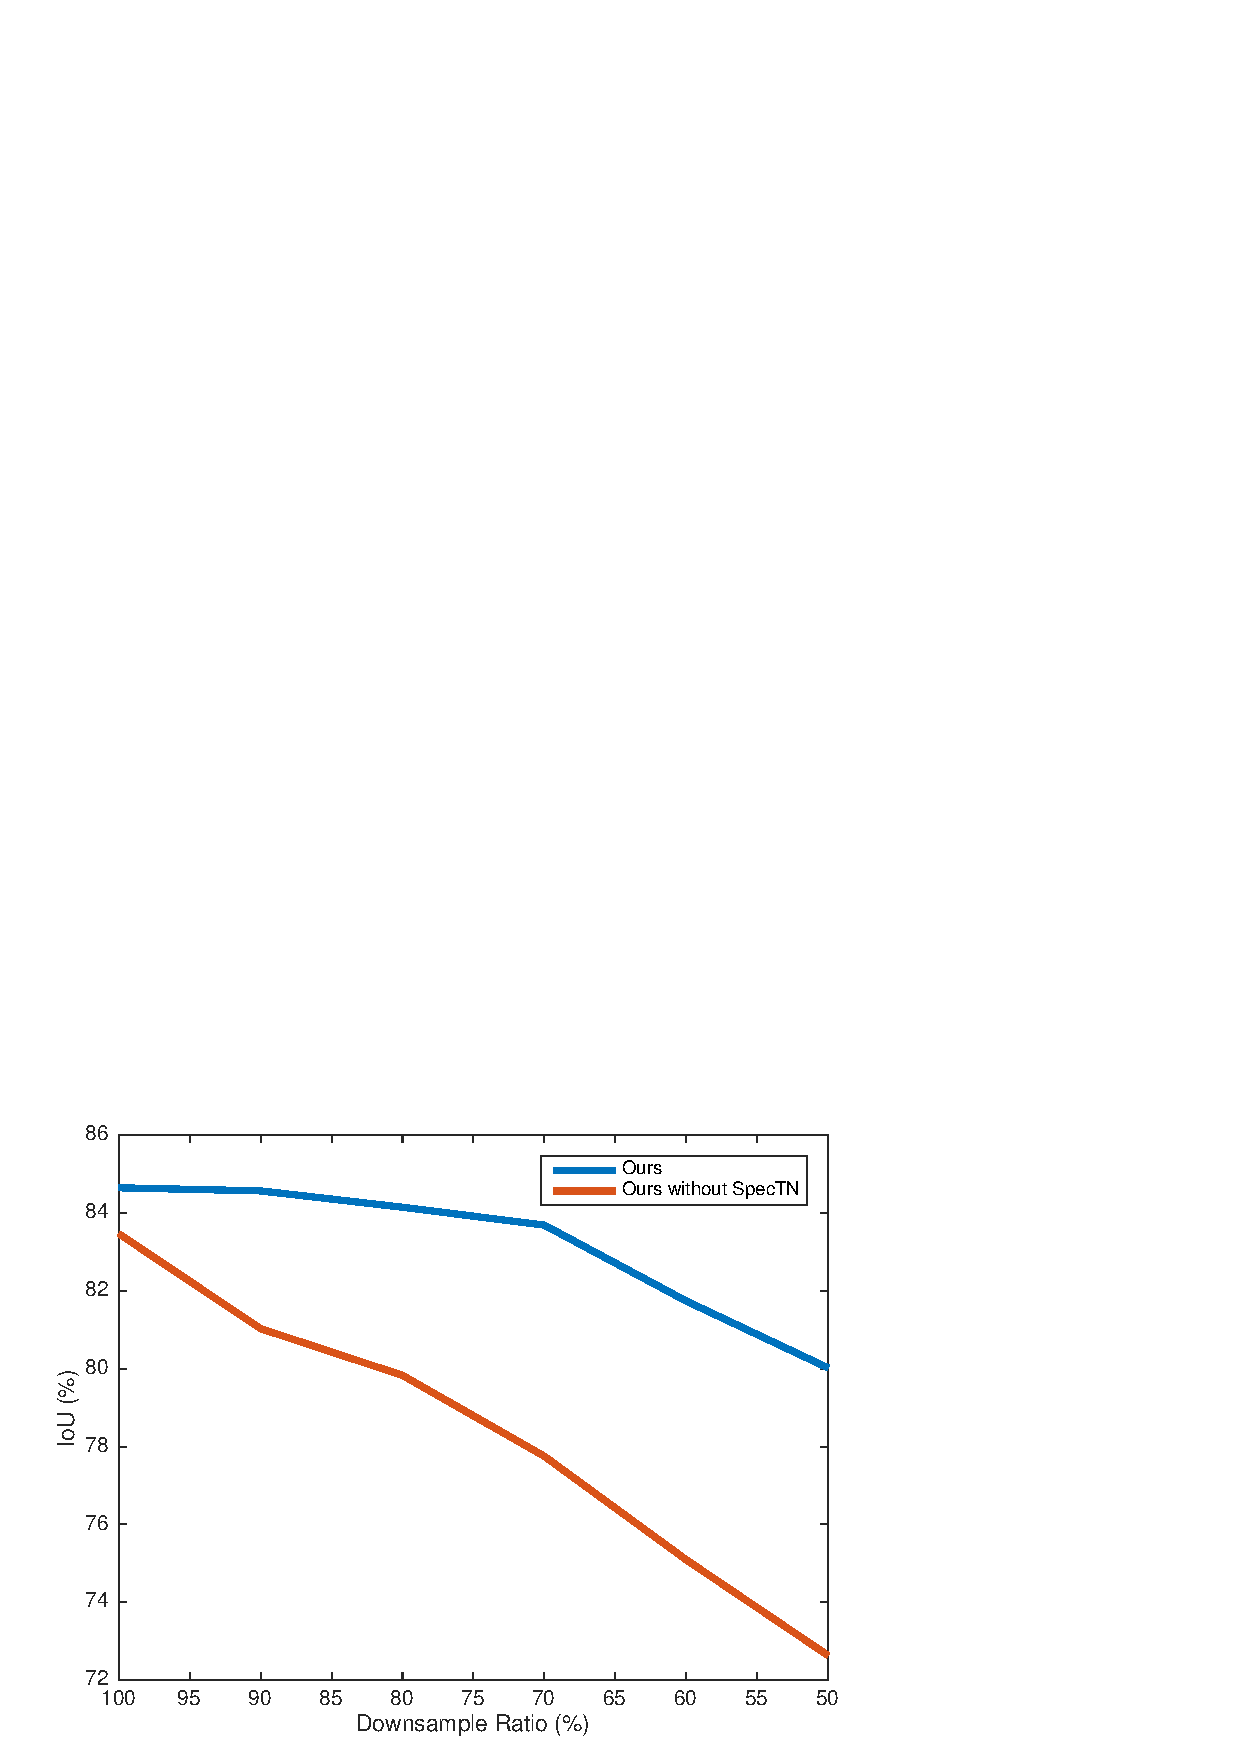
\includegraphics[width=0.8\linewidth]{./fig/downsample.pdf}
 \caption{We evaluate the robustness of our model to sampling density change. Test shapes are downsampled by different ratios and fed into our network. We compute the segmentation IoU for different downsample ratios and show it here. With SpecTN, our framework becomes more robust to sampling density change.}
 \label{fig:downsample}
\end{figure}

%\todo{Visualize joint basis}

\subsection{Qualitative Results and Error Analysis}
Figure~\ref{fig:erroranalysis} shows segmentation results generated from our network on two categories, Chair and Lamp. Representative good results are shown in the first block and  typical error patterns are summarized from the second to fourth blocks.

Most of our segmentation is very close to ground truth as is shown in the first block. We can accurately segment shapes with large geometric or topological variations like wide bench v.s. ordinary chair, pendant lamp v.s. table lamp. The lamp base on the first row and the lampshade on the second row are very similar regarding their local geometry; however, since our network is able to capture large scale context information, it could still differentiate the two and segment shapes correctly.

We observe several typical error patterns in our results. Most segmentation error occurs along part boundaries. %Our network sometimes generates fuzzy part boundaries, especially if the underlying part segments have a very smooth normal transition, as is shown in the second row of the second block. 
There are also cases where the semantic definition of parts has inherent ambiguities. %In these cases, our network may generate predictions slightly different from the ground truth but are still reasonable. 
We also observe a third type of error pattern, in which our prediction might miss a certain part completely, as is shown in the fourth block.

\begin{figure}
    \centering
    \includegraphics[width=\linewidth]{./fig/erroranalysis4.pdf}
    \caption{We visualize some segmentation results from our network prediction. The first block shows typical correct segmentations, notice the huge shape variation we can cover. The second to fourth blocks summarize different error patterns we observe in the results.}
    \label{fig:erroranalysis}
\end{figure}

\iffalse
\todo{
Compare different alternatives of our method
\begin{itemize}
    \item with multiple representatives instead of a single canonical space for spectral synchronization
    \item without join basis learning, visualize joint basis
    \item without dilated kernel, visualize dilated kernel
    \item different kernel choice: polynomial, cubic splines, exponential window, modulated exponential window
    \item different input vertex functions, extrinsic vertex functions help much since it's essentially a combination between extrinsic and intrinsic information for segmentation. intrinsic feature might not help much since the network is intrinsic and captures quite a lot intrinsic information already.
    \item network design, with/without skip link
\end{itemize}
}
\fi

\vspace{-8pt}
\section{Conclusions}



In this paper, we first examined the importance of introducing an intermediate attribute prediction layer into the predominant CNN-LSTM framework,
which was neglected by almost all previous work.
We implemented an attribute-based model which can be applied to the task of image captioning. We have shown that an explicit representation of image content improves \V2L performance, in all cases. Indeed, at the time of submitting this paper,
our image captioning model outperforms the state-of-the-art on several captioning datasets.



Secondly, in this paper we have shown that it is possible to extend the state-of-the-art RNN-based VQA approach so as to incorporate the large volumes of information required to answer general, open-ended, questions about images. The knowledge bases which are currently available do not contain much of the information which would be beneficial to this process, but nonetheless can still be used to significantly improve performance on questions requiring external knowledge (such as 'Why' questions).  The approach that we propose is very general, however, and will be applicable to more informative knowledge bases should they become available. We further implement a knowledge selection scheme which reflects both of the content of the question and the image, in order to extract more specifically related information. Currently our system is the state-of-the-art on three VQA datasets and produces the best results on the VQA evaluation server.

Further work includes generating knowledge-base queries which reflect the content of the question and the image, in order to extract more specifically related information. The Knowledge Base itself also can be improved. For instance, Open-IE provides more general common-sense knowledge such as `cats eat fish'. Such knowledge will help answer high-level questions.

%
%
%
%
%
%
%
%
%
%
%
%
%
%
%
%
%
%
%
%
%
%
%
%

\begin{table}[t!]
\centering
\scriptsize
\resizebox{\linewidth}{!}{
\begin{tabular}{lccclc}
\Xhline{2\arrayrulewidth}
\multicolumn{1}{c}{VQA}& \multicolumn{3}{c}{Answer Type} &  & Overall \\ \cline{2-4}
\multicolumn{1}{c}{Test-standard} & Yes/No & Other & Number &  &  \\ \hline
LSTM Q \cite{antol2015vqa}& 78.12 & 26.99 & 34.94 &  & 48.89 \\
LSTM Q+I \cite{antol2015vqa}& 79.01 & 36.80 & 35.55 &  & 54.06 \\
IBOWING \cite{zhou2015simple}&76.76&42.62&34.98&&55.89\\
NMN \cite{andreas2015deep}& 81.16 & 44.01 & 37.70 &  & 58.66\\
DNMN \cite{andreas2016learning}&80.98&45.81&37.48&&59.44\\
SMem \cite{xu2015ask}&80.80&43.48&37.53&&58.24\\
SAN \cite{yang2015stacked}& 79.11 & 46.42 &36.41  &  & 58.85\\
DDPnet\cite{Noh2015image}&80.28&42.24&36.92&&57.36\\
Human \cite{antol2015vqa}&95.77&72.67&83.39&&83.30\\
\hline
Ours & 81.10 & 45.90 & 37.18 &  & \textbf{59.50} \\ \Xhline{2\arrayrulewidth}
\end{tabular} }
\vspace{-3pt}
\caption{VQA Open-Ended evaluation server results. Accuracies for different answer types and overall performances on the test-standard. We only list the published results before this submission, the whole list of the leanding board can be found from http://www.visualqa.org/roe.html}
\vspace{-12pt}
\label{tab:server_results_2}
\end{table}

\vspace{-7pt}
\section*{Acknowledgements}
This research was in part supported by the Data to Decisions Cooperative Research Centre.
Correspondence should be addressed to C. Shen.
%



\begin{figure*}[t]
\resizebox{\linewidth}{!}{
\begin{tabular}{lcccc}
 \multicolumn{2}{c}{\includegraphics[height=3cm]{img/results/001.jpg}}&\includegraphics[height=3cm]{img/results/003.jpg}&\includegraphics[height=3cm]{img/results/006.jpg}&\includegraphics[height=3cm]{img/results/008.jpg}\\
 \multicolumn{2}{c}{What color is the tablecloth?}&How many people in the photo?&What is the red fruit?&What are these people doing?\\ \hline
 \textit{Ours:} &\color{green}{white}&\color{green}{2}&\color{green}{apple}&\color{green}{eating}\\
 \textit{Vgg+LSTM:} &\color{red}{red}&\color{red}{1}&\color{red}{banana}&\color{red}{playing}\\
 \textit{Ground Truth:} &white&2&apple&eating\\ \Xhline{2\arrayrulewidth}
 \vspace{1pt}
\end{tabular}}
\resizebox{\linewidth}{!}{
\begin{tabular}{lcccc}
 \multicolumn{2}{c}{\includegraphics[height=3cm]{img/results/002.jpg}}&\includegraphics[height=3cm]{img/results/004.jpg}&\includegraphics[height=3cm]{img/results/005.jpg}&\includegraphics[height=3cm]{img/results/007.jpg}\\
 \multicolumn{2}{c}{Why are his hands outstretched?}&Why are the zebras in water?&Is the dog standing or laying down?&Which sport is this?\\ \hline
 \textit{Ours:} &\color{green}{balance}&\color{green}{drinking}&\color{green}{laying down}&\color{green}{baseball}\\
 \textit{Vgg+LSTM:} &\color{red}{play}&\color{red}{water}&\color{red}{sitting}&\color{red}{tennis}\\
 \textit{Ground Truth:} &balance&drinking&laying down&baseball\\ \Xhline{2\arrayrulewidth}
 \vspace{-3pt}
\end{tabular}}
%
%
%
%
%
%
%
%
%
%
%
%
%
%
%
%
%
%
%
%
%
%
%
%
%
%
%
\vspace{-7pt}
\caption{Some example cases where our final model gives the correct answer while the base line model \textbf{VggNet-LSTM} generates the wrong answer. All results are from the VQA dataset. More results can be found in the supplementary material.}
\label{results_examples}
\vspace{-15pt}
\end{figure*}
\ifCLASSOPTIONcaptionsoff
  \newpage
\fi
%
%

\bibliographystyle{IEEEtran}
%
\bibliography{IEEEabrv,./myref}

%
%
%

\vspace{-1cm}
\begin{wrapfigure}{l}{7em}
\vspace{-10pt}
  \includegraphics[width=7em]{author-wu_bw.jpg}
\end{wrapfigure}
\begin{IEEEbiographynophoto}{Qi Wu}
is a postdoctoral researcher at the Australian Centre for Visual Technologies (ACVT) of the University of Adelaide. His research interests include cross-depiction object detection and classification, attributes learning, neural networks, and image captioning. He received a Bachelor in mathematical sciences from China Jiliang University, a Masters in Computer Science, and a PhD in computer vision from the University of Bath (UK) in 2012 and 2015, respectively.
\end{IEEEbiographynophoto}

\vspace{-1cm}
\begin{wrapfigure}{l}{7em}
\vspace{-10pt}
  \includegraphics[width=7em]{author-shen.jpg}
\end{wrapfigure}
\begin{IEEEbiographynophoto}{Chunhua Shen}
is a Professor of computer science at the University of Adelaide. He was with the computer vision program at NICTA (National ICT Australia) in Canberra for six years before moving back to Adelaide. He studied at Nanjing University (China), at the Australian National University, and received his PhD degree from the University of Adelaide. In 2012, he was awarded the Australian Research Council Future Fellowship.
\end{IEEEbiographynophoto}

\vspace{-1cm}
\begin{wrapfigure}{l}{7em}
\vspace{-10pt}
  \includegraphics[width=7em]{author-wang_bw.jpg}
\end{wrapfigure}
\begin{IEEEbiographynophoto}{Peng Wang}
is a postdoctoral researcher at the Australian Centre for Visual Technologies (ACVT) of the University of Adelaide. He received a Bachelor in electrical engineering and automation, and a PhD in control science and engineering from Beihang University (China) in 2004 and 2011, respectively.
\end{IEEEbiographynophoto}

\vspace{-0.5cm}
\begin{wrapfigure}{l}{7em}
\vspace{-10pt}
  \includegraphics[width=7em]{author-dick.png}
\end{wrapfigure}
\begin{IEEEbiographynophoto}{Anthony Dick}
is an Associate Professor at the University of Adelaide. He
received a PhD degree from the University of Cambridge in 2002, where he worked on 3D reconstruction of architecture from images. His research interests include image-based modeling, automated video surveillance, and image search.
\end{IEEEbiographynophoto}

\vspace{-0.5cm}
\begin{wrapfigure}{l}{7em}
\vspace{-10pt}
  \includegraphics[width=7em]{author-hengel.png}
\end{wrapfigure}
\begin{IEEEbiographynophoto}{Anton van den Hengel}
is a Professor at the University of Adelaide and the founding Director of The Australian Centre for Visual Technologies (ACVT). He received a PhD in Computer Vision in 2000, a Master Degree in Computer Science in 1994, a Bachelor of Laws in 1993, and a Bachelor of Mathematical Science in 1991, all from The University of Adelaide.
\end{IEEEbiographynophoto}

\end{document}





%
%
%
%
